\documentclass[a4paper,11pt]{article}
\usepackage[british]{babel}
\usepackage{fullpage}
\usepackage{amsmath,amssymb}
\usepackage{multirow}
\usepackage{caption}
\usepackage{tikz,pgfplots}
\usepackage{hyperref}
\usepackage{graphicx}

\title{\textbf{Low-level Parallel Programming (course 1DL550) \\
    Uppsala University -- Spring 2015 \\
    Report for Lab 1 by Team 14}}
\author{Fredrik Larsson \and Jimmy Holm \and Per Bergqwist}
\date{\today}

\begin{document}
\maketitle

\section{}
\begin{center}
  \pgfplotsset{grid style={dotted,gray}}
  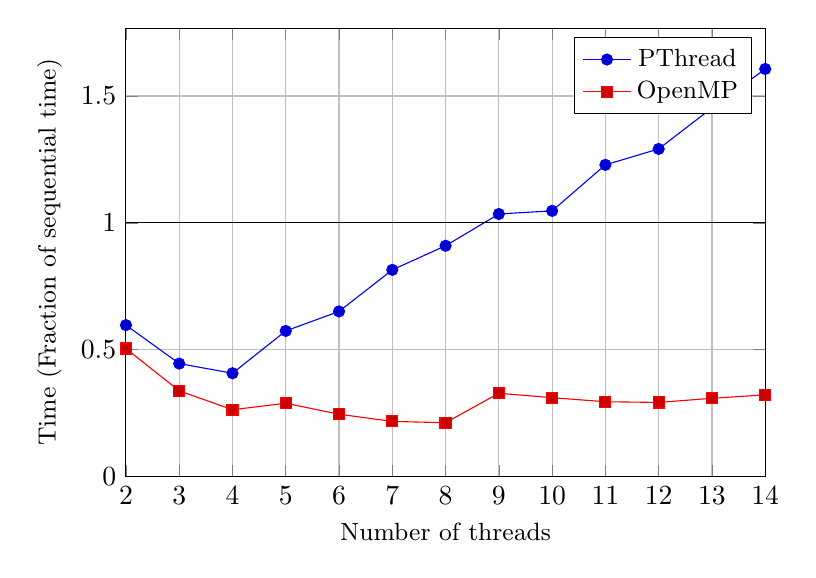
\begin{tikzpicture}
    \begin{axis}[
        width=0.8\textwidth,
        height=0.6\textwidth,
        xtick={2,...,14},
        xmin=2,
        xmax=14,
        ymin=0,
        grid=both,
        legend entries={\small PThread,\small OpenMP},
        xlabel={\small Number of threads},
        ylabel={\small Time (Fraction of sequential time)}
      ]
      \addplot coordinates{
        (2,0.596941)
        (3,0.445256)
        (4,0.407209)
        (5,0.573977)
        (6,0.650869)
        (7,0.814665)
        (8,0.909659)
        (9,1.0349)
        (10,1.04726)
        (11,1.22862)
        (12,1.29125)
        (13,1.45297)
        (14,1.60644)};
      \addplot coordinates{
        (2,0.504375)
        (3,0.337991)
        (4,0.263352)
        (5,0.288928)
        (6,0.245644)
        (7,0.217354)
        (8,0.21215)
        (9,0.328347)
        (10,0.310834)
        (11,0.294817)
        (12,0.292123)
        (13,0.308487)
        (14,0.322058)};
      \draw (axis cs:2,1) -- (axis cs:14,1);%2.864929
    \end{axis}
  \end{tikzpicture}
\end{center}

\end{document}
